%% Use the option review to obtain double line spacing
 \documentclass[review,1p]{elsarticle}

%% Use the options 1p,twocolumn; 3p; 3p,twocolumn; 5p; or 5p,twocolumn
%% for a journal layout:
%% \documentclass[final,1p,times]{elsarticle}
%%\documentclass[final,1p,times,twocolumn]{elsarticle}
%% \documentclass[final,3p,times]{elsarticle}
%% \documentclass[final,3p,times,twocolumn]{elsarticle}
%% \documentclass[final,5p,times]{elsarticle}
%% \documentclass[final,5p,times,twocolumn]{elsarticle}

%% The graphicx package provides the includegraphics command.
\usepackage{graphicx}
%% The amssymb package provides various useful mathematical symbols
\usepackage{amssymb}
\usepackage{amsmath}
\usepackage{siunitx}
%% The amsthm package provides extended theorem environments
%% \usepackage{amsthm}

%% The lineno packages adds line numbers. Start line numbering with
%% \begin{linenumbers}, end it with \end{linenumbers}. Or switch it on
%% for the whole article with \linenumbers after \end{frontmatter}.
\usepackage{lineno}

%% natbib.sty is loaded by default. However, natbib options can be
%% provided with \biboptions{...} command. Following options are
%% valid:

%%   round  -  round parentheses are used (default)
%%   square -  square brackets are used   [option]
%%   curly  -  curly braces are used      {option}
%%   angle  -  angle brackets are used    <option>
%%   semicolon  -  multiple citations separated by semi-colon
%%   colon  - same as semicolon, an earlier confusion
%%   comma  -  separated by comma
%%   numbers-  selects numerical citations
%%   super  -  numerical citations as superscripts
%%   sort   -  sorts multiple citations according to order in ref. list
%%   sort&compress   -  like sort, but also compresses numerical citations
%%   compress - compresses without sorting
%%
%% \biboptions{comma,round}

% \biboptions{}

\begin{document}

\makeatletter
\def\ps@pprintTitle{%
  \let\@oddhead\@empty
  \let\@evenhead\@empty
  \let\@oddfoot\@empty
  \let\@evenfoot\@oddfoot
}
\makeatother

\begin{frontmatter}

%% Title, authors and addresses

\title{Transformada de Fourier}

%% use the tnoteref command within \title for footnotes;
%% use the tnotetext command for the associated footnote;
%% use the fnref command within \author or \address for footnotes;
%% use the fntext command for the associated footnote;
%% use the corref command within \author for corresponding author footnotes;
%% use the cortext command for the associated footnote;
%% use the ead command for the email address,
%% and the form \ead[url] for the home page:
%%
%% \title{Title\tnoteref{label1}}
%% \tnotetext[label1]{}
%% \author{Name\corref{cor1}\fnref{label2}}
%% \ead{email address}
%% \ead[url]{home page}
%% \fntext[label2]{}
%% \cortext[cor1]{}
%% \address{Address\fnref{label3}}
%% \fntext[label3]{}


%% use optional labels to link authors explicitly to addresses:
%% \author[label1,label2]{<author name>}
%% \address[label1]{<address>}
%% \address[label2]{<address>}

\author{Gabriel Alexander Valdivia Medina, Giulia Alexa Naval Fernandez, Rodrigo Alonso Torres Sotomayor}

\address{Universidad Católica San Pablo, Arequipa.}

\begin{abstract}
Este trabajo está orientado en presentar la Tranformada de Fourier(TF),
explicar su funcionamiento, capacidades y versiones, así como proponer un
algoritmo en el lenguaje de programación C++ para su uso práctico. Se implementará 
una aplicación típica del algoritmo a modo de ejemplificación de lo que se puede
lograr con este. 
\end{abstract}

\begin{keyword}
Trasformada de Fourier \sep solution \sep degree of a polynomial \sep linear 
\sep quadratic \sep quadratic formula \sep roots \sep cubics \sep quartics
%% keywords here, in the form: keyword \sep keyword

%% MSC codes here, in the form: \MSC code \sep code
%% or \MSC[2008] code \sep code (2000 is the default)

\end{keyword}

\end{frontmatter}

%%
%% Start line numbering here if you want
%%

%% main text
\section{La Serie de Fourier}

\[
    P(x) = a_0 + a_1x + a_2x^2 + ...  + a_ix^i
\]

\section{Transformada de Fourier}
La transformada de Fourier nos permite, entre muchas cosas, cambiar la forma en 
la que miramos una señal o potencia, pasando de mirar su comportamiento en 
base de tiempo a verla en base a su frecuencia.\\
Se relaciona con la Serie de Fourier, ya puede representar todas las
amplitudes de las curvas encontradas en esta serie.\\
\begin{figure}[h]
    \centering
    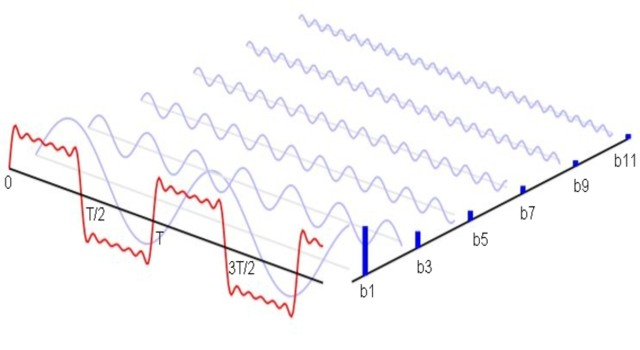
\includegraphics[scale=0.5]{Figuras/Serie-transformada.jpg}
    %%\medskip
    \\
    \small Figura1. En rojo, la señal recibida. En azul intenso, la transformada
    de Fourier. En morado, las series de Fourier. Fuente: wikimedia commons.\\
\end{figure}\\
La transformada se halla con el producto interno entre la señal recibida y una
exponencial compleja de frecuencia fija:\\
\begin{equation}
    X(f) = \int_{- \infty}^{\infty} X(t) \cdot e^{-2\pi ift} dt 
\end{equation}
Donde $X(t)$ es la señal en base tiempo definida, $X(f)$ la vista en base frecuencia
que se busca. El cambio más común es de tiempo a frecuencia, pero no es el único que la 
transformada puede manejar.\\
\subsection{Ejemplo 1}
Hallaremos la transformada de la siguiente función:\\
\begin{figure}[h]
    \centering
    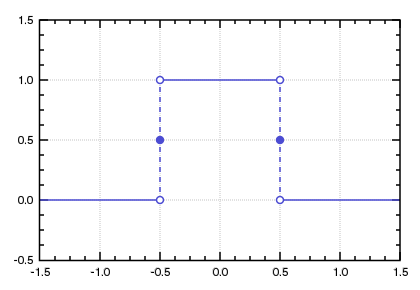
\includegraphics[scale=0.5]{Figuras/Funcion_cajon.png}
    \\
    \small Figura 2. Función rectangular, función cajón, o pulso unitario.\\
\end{figure}\\
Para hallar la transformada de una función por partes, se hallan las transformadas
de las partes por separado:\\
\[
    X(f) = \int_{- \infty}^{-0.5} rect(t) \cdot e^{-2\pi ift} dt +
    \int_{-0.5}^{0.5} rect(t) \cdot e^{-2\pi ift} dt + 
    \int_{0.5}^{\infty} rect(t) \cdot e^{-2\pi ift} dt
\]
\\
Sin embargo, dado que $rect(t)$ es igual a 0 tanto en la primera como en la
tercera parte, nos quedamos sólo con la transformada del medio.\\
\[
    X(f) = \int_{-0.5}^{0.5} 1\cdot e^{-2\pi ift} dt
\]
Desarrollamos la integral:\\
\[
    X(f) = [\frac{e^{-i2\pi ft}}{-i2\pi f}]_{-0.5}^{0.5}
\]
\[
    X(f) = \frac{e^{-i\pi f} - e^{i\pi f} }{-2\pi fi}  
\]
Por teoría de números complejos, sabemos que las funciones $sen$ y $cos$ se
relacionan con las funciones exponenciales de la forma:\\
\begin{equation}
    cos(\theta) = \frac{1}{2}(e^{+i\theta}+e^{-i\theta})
\end{equation}
\begin{equation}
    sen(\theta) = \frac{1}{2i}(e^{+i\theta}-e^{-i\theta})
\end{equation}
Entonces, pordemos acomodar nuestra ecuación para que satisfaga alguna:\\
\begin{align*}
    X(f) = \frac{-e^{-i\pi f} + e^{i\pi f}}{2i} \cdot \frac{1}{\pi f}\\
    X(f) = \frac{sen(\pi f)}{\pi f}  \\
    X(f) = sinc(\pi f)\\
\end{align*}
  
  

\section{Tranformada Inversa de Fourier}
La transformada inversa de Fourier, básicamente, revierte el estado en que se encuentra la representación de una onda luego de aplicarle la Transformada de Fourier normal. De forma más específica, convierte una serie de tamaño potencia de 2 de números complejos, puntos en el espectro de frecuencia, en una serie del mismo tamaño en un dominio de tiempo.\\

\section{Algoritmo Cooley-Tukey}
Pensando en formas de implementar y mejorar la TFD, James W. Cooley y John W. Tukey publicaron en su paper insigne en 1965 una implementación de la transformada utilizando el paradigma "divide y vencerás", denominada como Transformada Rápida de Fourier. En dicho trabajo, se destaca la ventaja que presenta el algoritmo en arreglos de tamaño N potencia de 2 sobre otros con N distintos, al lograr una complejidad de $O(Nlog(N))$ para el primer caso. \\

Este algoritmo consigue reducir el número de cálculos al dividir el arreglo de tamaño N del polinomio en 2 de tamaño N/2, uno con el contenido de los índices impares y el otro con el de los índices pares. \\
\begin{figure}[ht]
    \centering
    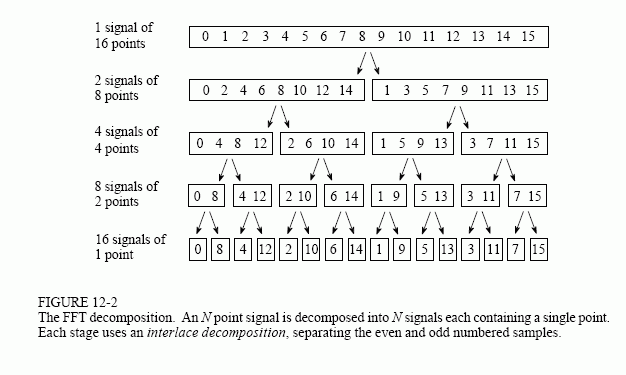
\includegraphics[scale=0.9]{Figuras/F_12_2.png}
    %%\medskip
    \\
    \small Figura3. Descomposición de arreglo de coeficientes del polinomio. Fuente: The Scientist and Engineer's Guide to Digital Signal Processing.
\end{figure}\\
Esta distribución también se puede lograr a través usando inversión de bits.\\
\begin{figure}[h]
    \centering
    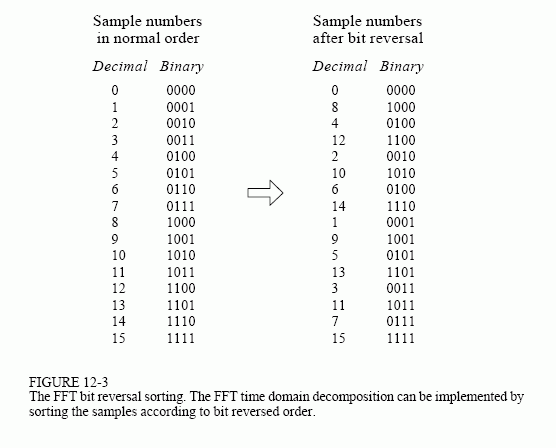
\includegraphics[scale=0.9]{Figuras/F_12_3.png}
    %%\medskip
    \\
    \small Figura4. Ordenamiento por inversión de bits. Fuente: The Scientist and Engineer's Guide to Digital Signal Processing.
\end{figure}
Una vez dividido el arreglo en partes más pequeñas, el algoritmo busca encontrar su valor en el espectro de frecuencia, donde obviamente, la frecuencia de las divisiones más pequeñas, es decir de 1 solo punto, será igual a sí mismo. Luego de esto, tendrá que regresar y juntar los resultados en el orden inverso al que se hicieron las divisiones. Para sumar los puntos de cada una, también se tienen que diluir la señal completando con 0s las posiciones pares o impares, dependiendo del sub-arreglo, lo que equivale a una duplicación de la data de la señal en el dominio de la frecuencia. Esta discordancia en la separación con 0s, o de forma más precisa, este corrimiento del segundo sub-arreglo corresponde a la multiplicación del mismo por un sinusoide. 
\clearpage
\begin{figure}[h!]
    \centering
    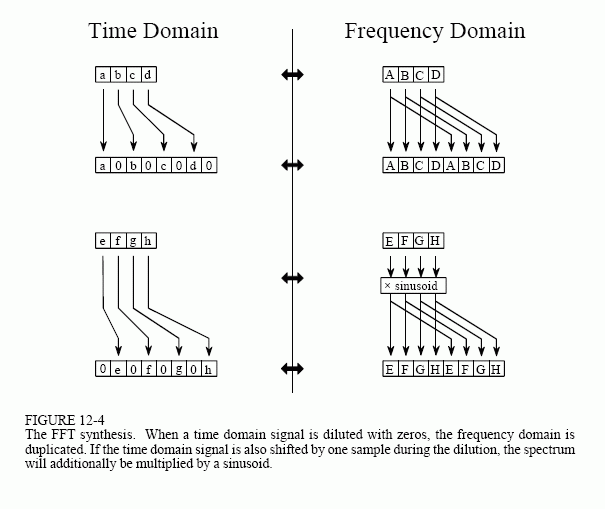
\includegraphics[scale=0.9]{Figuras/F_12_4.png}
    %%\medskip
    \\
    \small Figura5. Separación de puntos con 0s y multiplicación por sinusoides. Fuente: The Scientist and Engineer's Guide to Digital Signal Processing.
\end{figure}
Esta forma de sumar los puntos del espectro mientras se los reordena, tiene el nombre de \textbf{mariposa} y es la operación base de toda la TFR. \\

\begin{figure}[!h]
    \centering
    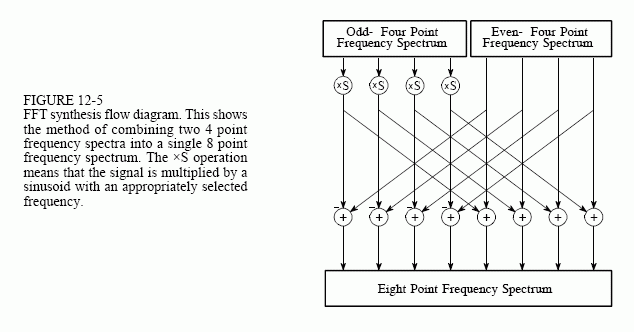
\includegraphics[scale=0.7]{Figuras/F_12_5.png}
    %%\medskip
    \\
    \small Figura6. Flujo cruzado de operaciones o \textit{mariposas}. Fuente: The Scientist and Engineer's Guide to Digital Signal Processing.\\
\end{figure}


\section{Algoritmo ...}
\section{Comparación de algoritmos}
\section{Aplicación Práctica: manipulación de audios usando la transformada de Fourier}
\section{Aplicación Práctica: procesado de imágenes usando la transformada de Fourier}

\section*{Apéndice}
A field is a set on which the binary operations $+$, $-$, $\times$ and $\div$ are defined.
Besides integral fields, there are other fields where polynomials will behave differently and a polynomial with finite terms and of a finite degree can also have infinite solutions.
%% The Appendices part is started with the command \appendix;
%% appendix sections are then done as normal sections
%% \appendix

%% \section{}
%% \label{}

%% References
%%
%% Following citation commands can be used in the body text:
%% Usage of \cite is as follows:
%%   \cite{key}          ==>>  [#]
%%   \cite[chap. 2]{key} ==>>  [#, chap. 2]
%%   \citet{key}         ==>>  Author [#]

%% References with bibTeX database:

%%\bibliographystyle{model1-num-names}
\appendix
\section*{Bibliography}
http://www.ijsea.com/archive/volume2/issue7/IJSEA02071002.pdf\\
http://people.scs.carleton.ca/~maheshwa/courses/5703COMP/16Fall/FFT\_Report.pdf\\
%%\bibliography{}

%% Authors are advised to submit their bibtex database files. They are
%% requested to list a bibtex style file in the manuscript if they do
%% not want to use model1-num-names.bst.

%% References without bibTeX database:

% \begin{thebibliography}{00}

%% \bibitem must have the following form:
%%   \bibitem{key}...
%%

% \bibitem{}

% \end{thebibliography}


\end{document}

%%
%% End of file `elsarticle-template-1-num.tex'.
